ss[department=cls, notes={hide notes}, official=true, grouplogo=lama]{beamerruhuisstijl}

\title{$p(\text{conclusions} | \text{Skipping \{*2*\}})$}
\subtitle{Bayesian Language Modelling with Skipgrams}
\date{\today}
\author{lama-fan}

\usepackage{cleveref}

\usepackage{tikz}
\usepackage{tkz-graph}
\usetikzlibrary[shapes,arrows,positioning,calc,patterns]

\usepackage{pgfplots}
\usepackage{pgfplotstable}
\pgfplotsset{compat=1.10}

\begin{document}

\begin{frame}
    \titlepage
\end{frame}
\note{

}

\begin{frame}{Bayesian Language Modelling with Skipgrams}
    \begin{block}{}
        Louis Onrust \\
        Centre for Language Studies, Radboud University \\
        Center for Processing Speech and Images, KU Leuven
    \end{block}

    \begin{block}{}
        \href{mailto:l.onrust@let.ru.nl}{l.onrust@let.ru.nl} \\
        \href{https://github.com/naiaden}{github.com/naiaden}
    \end{block}
\end{frame}
\note[itemize]{
}

\begin{frame}{Language Models}
    \begin{block}{Applications}
        \begin{itemize}
            \item Input assists on telephones
            \item Automatic translation of search results
            \item Digital court reporting
        \end{itemize}
    \end{block}
    
    \uncover<2->{
    \begin{block}{Flavours}
      \begin{itemize}
          \item Frequentist language models
          \item Bayesian language models
          \item Neural language models
          \item \ldots
      \end{itemize}
    \end{block}
    }
\end{frame}
\note{

}

\begin{frame}{The Task at Hand}
    \begin{center}
        \emph{After all , tomorrow is another [\ldots]}
    \end{center}

    \begin{columns}[T] 
        \uncover<2->{
        \begin{column}[T]{0.25\textwidth} 
            \begin{block}{Word prediction}
                \uncover<3->{
                \begin{itemize}
                    \item day
                \end{itemize}   
                }
            \end{block}
        \end{column}
   % }
   
        \begin{column}[T]{0.25\textwidth} 
            \begin{block}{Word probability}
                 \uncover<4->{
                \begin{itemize}
                    \item cow
                    \item day
                    \item vegetable
                    \item \ldots
                \end{itemize}
                }
            \end{block}
        \end{column}
        
        \begin{column}[T]{0.45\textwidth} 
            \begin{block}{Pattern probability}
                 \uncover<5->{
                \begin{itemize}
                    \item tomorrow is another day
                    \item tomorrow is another important
                    \item tomorrow is another race
                \end{itemize}
                }
            \end{block}
        \end{column}
    }
    \end{columns}
    
\pgfplotstableread[col sep=comma,header=true,row sep=crcr]{
word,freq\\
day,11\\
important,1\\
race,1\\
}\data
% \begin{center}
\medskip
\uncover<4->{
    \begin{tikzpicture}     
        \begin{axis}[    
            width=8cm,
            height=3.5cm,
            xbar,                                 
            xtick={0,5,10,15},    
            xmin=0,
            xmax=15,  
            nodes near coords, nodes near coords align={horizontal},
            symbolic y coords={day,important,race},
            xlabel={Observed frequency},
            y label style={at={(-0.1,0.5)}},
            enlarge x limits={abs=0},
            reverse legend,
        ]
        \addplot table [x=freq, y=word] {\data};
        \end{axis}
    \end{tikzpicture}
}
% \end{center}
\end{frame}

\begin{frame}{Generalising the $n$-gram}
    \begin{block}{$n$-grams}
        \begin{itemize}
            \item Continuous sequence of $n$ words
        \end{itemize}
    \end{block}
    
    \begin{block}{Skipgrams}
        \begin{itemize}
            \item $n$-gram with at most $n-2$ skips of length 1
        \end{itemize}
    \end{block}
    
    \begin{block}{Flexgrams}
        \begin{itemize}
            \item $n$-gram with any number of skips of any length
        \end{itemize}
    \end{block}
    \bigskip
    \begin{block}{Skipgrams in RNN}
        \begin{itemize}
            \item Based on embeddings rather than co-occurrence
            \item Co-occurrence of embeddings
        \end{itemize}
    \end{block}
\end{frame}

\begin{frame}{Backoff Patterns with Skipgrams}
     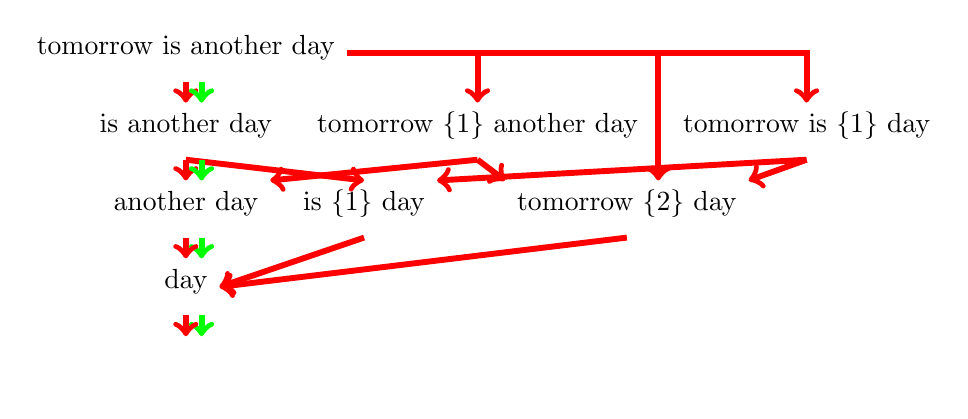
\begin{tikzpicture}[->,auto, node distance=0.75em,text centered,text height=1.5ex,text depth=1.25ex,line width=0.75mm]
    \node (abcd) {tomorrow is another day};
    
    
    \node[below = of abcd] (bcd) {is another day}; 
    \node[right = of bcd] (axcd) {tomorrow \{1\} another day};
    \node[right = of axcd] (abxd) {tomorrow is \{1\} day};
    \node[below = of bcd] (cd) {another day};
    
    \node[right = of cd] (bxd) {is \{1\} day};
    \node[below = of cd] (d) {day};
    \node[below = of d] (empty) {$\varnothing$};
    
    \node[xshift=0.6cm,right = of bxd] (axxd) {tomorrow \{2\} day};
    
    
    %%1
    
    \draw[red] let \p1 = (abcd.south), \p2 = (bcd.north) in (\x1,\y1) -- (\x2,\y2);
    \draw[red] let \p1 = (abcd.east), \p2 = (axcd.north) in (\x1,\y1) -| (\x2,\y2);
    \draw[red] let \p1 = (abcd.east), \p2 = (abxd.north) in (\x1,\y1) -| (\x2,\y2);
    \draw[red] let \p1 = (abcd.east), \p2 = ([xshift=0.4cm]axxd.north) in (\x1,\y1) -| (\x2,\y2);
    
    \draw[green] let \p1 = ([xshift=0.2cm]abcd.south), \p2 = ([xshift=0.2cm]bcd.north) in (\x1,\y1) -- (\x2,\y2);
    
%     \draw[blue] let \p1 = ([xshift=-0.2cm]abcd.south), \p2 = ([xshift=-0.2cm]bcd.north) in (\x1,\y1) -- (\x2,\y2);  
%     \draw[blue] let \p1 = ([yshift=0.2cm]abcd.east), \p2 = ([xshift=-0.2cm]axcd.north) in (\x1,\y1) -| (\x2,\y2);
%     \draw[blue] let \p1 = ([yshift=0.2cm]abcd.east), \p2 = ([xshift=-0.2cm]abxd.north) in (\x1,\y1) -| (\x2,\y2); 
%     \draw[blue] let \p1 = ([yshift=0.2cm]abcd.east), \p2 = ([xshift=0.2cm]axxd.north) in (\x1,\y1) -| (\x2,\y2);
    

    \draw[red] let \p1 = (axxd.south), \p2 = (d.east) in (\x1,\y1) -- (\x2,\y2);    
    
    
%     %%2
  
  \draw[red] let        \p1 = (bcd.south), \p2 = (cd.north) in (\x1,\y1) -- (\x2,\y2);
    \draw[red] let      \p1 = (bcd.south), 
                    \p2 = (bxd.north) in (\x1,\y1) -- (\x2,\y2);  
    \draw[red] let      \p1 = (axcd.south), 
                    \p2 = (cd.north east) in (\x1,\y1) -- (\x2,\y2);    
    \draw[red] let      \p1 = (abxd.south), 
                    \p2 = (bxd.north east)
                        in (\x1,\y1) -- (\x2,\y2);
%     \draw[red] let    \p1 = (bcd.south), \p2 = (cd.north) in (\x1,\y1) -- (\x2,\y2);
%     \draw[red] let    \p1 = (bcd.south), 
%                               \p2 = (bxd.north), 
%                     \p3 = ([yshift=-0.35cm]bcd.south), 
%                     \p4 = ([yshift=0.15cm]bxd.north) 
%                       in (\x1,\y1) -| (\x3,\y3) -| (\x4,\y4) -| (\x2,\y2);  
%     \draw[red] let    \p1 = ([xshift=-0.1cm]axcd.south), 
%                               \p2 = ([xshift=0.4cm]cd.north), 
%                     \p3 = ([xshift=-0.1cm,yshift=-0.15cm]axcd.south), 
%                     \p4 = ([xshift=0.4cm,yshift=0.15cm]cd.north) 
%                       in (\x1,\y1) -| (\x3,\y3) -| (\x4,\y4) -| (\x2,\y2);    
%     \draw[red] let    \p1 = (abxd.south), 
%                               \p2 = (bxd.east)
%                       in (\x1,\y1) |- (\x2,\y2);    
    
%     \draw[blue] let \p1 = ([xshift=-0.2cm]abxd.south), 
%                               \p2 = ([yshift=0.2cm]bxd.east)
%                       in (\x1,\y1) |- (\x2,\y2);
%     \draw[blue] let \p1 = ([xshift=-0.2cm]bcd.south), 
%                               \p2 = ([xshift=-0.2cm]bxd.north), 
%                     \p3 = ([xshift=-0.2cm,yshift=-0.27cm]bcd.south), 
%                     \p4 = ([xshift=-0.2cm,yshift=0.27cm]bxd.north) 
%                       in (\x1,\y1) -| (\x3,\y3) -| (\x4,\y4) -| (\x2,\y2);
                        
    \draw[red] let      \p1 = (axcd.south), 
                    \p2 = (axxd.north west) in (\x1,\y1) -- (\x2,\y2);
                        
    \draw[red] let      \p1 = (abxd.south), 
                    \p2 = (axxd.north east) in (\x1,\y1) -- (\x2,\y2);    
                        
%     \draw[blue] let \p1 = ([xshift=0.3cm]abxd.south), 
%                               \p2 = ([xshift=-0.2cm]axxd.north), 
%                     \p3 = ([xshift=0.3cm,yshift=-0.15cm]abxd.south), 
%                     \p4 = ([yshift=0.3cm,xshift=-0.2cm]axxd.north) 
%                       in (\x1,\y1) -| (\x3,\y3) -| (\x4,\y4) -| (\x2,\y2);                     
    
    
    \draw[green] let \p1 = ([xshift=0.2cm]bcd.south), \p2 = ([xshift=0.2cm]cd.north) in (\x1,\y1) -- (\x2,\y2);
%     \draw[blue] let \p1 = ([xshift=-0.2cm]bcd.south), \p2 = ([xshift=-0.2cm]cd.north) in (\x1,\y1) -- (\x2,\y2);

%  %%3 
   
   
     \draw[green] let \p1 = ([xshift=0.2cm]cd.south), \p2 = ([xshift=0.2cm]d.north) in (\x1,\y1) -- (\x2,\y2); 
     \draw[red] let \p1 = (cd.south), \p2 = (d.north) in (\x1,\y1) -- (\x2,\y2); 
     \draw[red] let  \p1 = (bxd.south), 
                     \p2 = (d.east)
                            in (\x1,\y1) -- (\x2,\y2);
%      \draw[blue] let \p1 = ([xshift=-0.2cm]bxd.south), 
%                                \p2 = ([yshift=0.2cm]d.east)
%                                               in (\x1,\y1) |- (\x2,\y2);
   
%    %%4
   
   
     \draw[green] let \p1 = ([xshift=0.2cm]d.south), \p2 = ([xshift=0.2cm]empty.north) in (\x1,\y1) -- (\x2,\y2);   
   \draw[red] let \p1 = (d.south), \p2 = (empty.north) in (\x1,\y1) -- (\x2,\y2);
   
   
   %%5
    
    
\end{tikzpicture}
\end{frame}

\begin{frame}{Probability Estimation}
    \begin{block}{Maximum Likelihood Estimate}
        \[ p_{\text{ML}}(w_i | w_{i-N+1},\ldots,w_{i-1}) = \frac{C(w_{i-N+1},\ldots,w_{i-1})}{C(w_{i-N+1},\ldots,w_{i})} \]
        \begin{itemize}
        \item Parameter estimation is impossible for $N>2$
        \item Na\"ive priors assuming independent parameters fail as well
        \end{itemize}
    \end{block}
    
    \uncover<2->{
    \begin{block}{Smoothing}
        \[ p_{\text{SM}}(w_i | w_{i-N+1},\ldots,w_{i-1}) = \sum_{n=1}^N\lambda(n)Q_n(w_i | w_{i-N+1},\ldots,w_{i-1}) \]
        \begin{itemize}
            \item Chen and Goodman found that interpolated and modified
Kneser-Ney are best under virtually all circumstances
        \end{itemize}
    \end{block}
    }
\end{frame}

\begin{frame}{Bayesian Probability Estimation}
    \begin{block}{Parametrise conditional probabilities}
    \vspace*{-1em}
        \[ p(w_i = w | w_{i-N+1},\ldots,w_{i-1} = u) = G_u(w)\]
        \[ G_u = [G_u(w)]_{w\in W} \] 
        \[ \pi(w_{i-N+1},\ldots,w_{i-1}) = w_{i-N+2},\ldots,w_{i-1} \] \vspace*{-1em}
        \begin{itemize}
            \item $G_u$ is a probability vector associated with context $u$
        \end{itemize}
    \end{block}
    
    \uncover<2->{
    \begin{block}{Hierarchical Dirichlet language model}
        \begin{itemize}
            \item What is $p(G_u|G_{\pi(u)})$?
            \item Standard Dirichlet distribution over probability vectors: does not outperform ikn and mkn (MacKay and Peto, 1994)
        \end{itemize}
    \end{block}
    }

    \uncover<3->{
    \begin{block}{Hierarchical Pitman-Yor process}
        \begin{itemize}
            \item Two-parameter extension of the Dirichlet distribution
            \item PYP produces power-law distributions
            \item Outperforms ikn and mkn (Teh, 2006)
        \end{itemize}
    \end{block}
    }
\end{frame}

\begin{frame}{Everlasting feud}
    \begin{columns}[T]
    \begin{column}[T]{0.45\textwidth}
    \begin{block}{Frequentists}
        \begin{itemize}
            \item Unconditional perspective: inferential methods should give good answers in repeated use
            \item ``pessimist'': let's protect ourselves against bad decisions given that our inferential procedure is inevitably based on a simplification of reality
            \item $R(\theta) = \mathbb{E}_\theta l(\delta(X),\theta)$
        \end{itemize}
    \end{block}
    \end{column}
    \begin{column}[T]{0.45\textwidth}
    \begin{block}{Bayesians}
    \begin{itemize}
            \item Conditional perspective: inferences should be made conditional on the current data
            \item ``optimistic'': let's make the best possible use of our sophisticated inferential tool
            \item $\rho(X) = \mathbb{E}[l(\delta(X),\theta)|X]$
        \end{itemize}
        
    \end{block}
    \end{column}
    \end{columns}
    
%     \begin{block}{Non-conformists}
%       \begin{itemize}
%               \item Choose the best solution given a problem
%         \end{itemize}
%     \end{block}

\end{frame}

\begin{frame}{Comparing HPYLM to MKN: the Numbers}
        The reported values are entropy values
        
        \begin{columns}[b]
            \begin{column}[b]{0.45\textwidth}
                \begin{block}{HPYLM}
                \begin{tabular}{lllllllll}
                         & jrc  & 1bw   & emea  & wp        \\
                    jrc  & 3.65 & 10.56 & 10.08 & 10.34     \\
                    1bws & 9.58 & 7.31  & 9.89  & 8.94      \\  
                    emea & 9.59 & 10.60 & 1.88  & 10.10     \\ 
                    wps  & 9.12 & 8.83  & 9.97  & 7.76      \\
                \end{tabular}
                \end{block}
                \vspace{0pt}
            \end{column}
            \quad
            \begin{column}[b]{0.45\textwidth}
                \begin{block}{Modified Kneser-Ney}
                \begin{tabular}{llll}
                    jrc   & 1bw   & emea  & wp    \\
                    4.43  & 10.70 & 10.35 & 10.84 \\
                    10.51 & 7.72  & 10.57 & 9.96  \\
                    10.12 & 10.77 & 3.28  & 10.70 \\
                    9.72  & 9.23  & 10.63 & 8.81  \\
                \end{tabular}
                \end{block}
                \vspace{0pt}
            \end{column}            
        \end{columns}
 
        \begin{columns}[b]
            \begin{column}[b]{0.45\textwidth}
                \begin{block}{Relative reduction in entropy (in \%)}
                \begin{tabular}{lllll}
                    jrc  & 17.66 & 1.31 & 2.67  & 4.67  \\
                    1bws & 8.82  & 5.37 & 6.44  & 10.19 \\
                    emea & 5.30  & 1.57 & 42.51 & 5.65  \\
                    wps  & 6.20  & 4.28 & 6.23  & 11.92 \\
                \end{tabular}
                \end{block}
                \vspace{0pt}
            \end{column}
            \quad
            \begin{column}[b]{0.45\textwidth}
                \begin{block}{Relative reduction in perplexity (in \%)}
                \begin{tabular}{llll}
                    41.87 & 9.25  & 17.43 & 29.63 \\
                    47.41 & 24.99 & 37.62 & 50.51 \\
                    31.04 & 11.08 & 61.92 & 34.27 \\
                    34.14 & 23.95 & 36.81 & 51.72 \\ 
                \end{tabular}
                \end{block}
                \vspace{0pt}
            \end{column}            
        \end{columns}

\end{frame}

\begin{frame}{Comparing HPYLM to MKN: the Figure}
    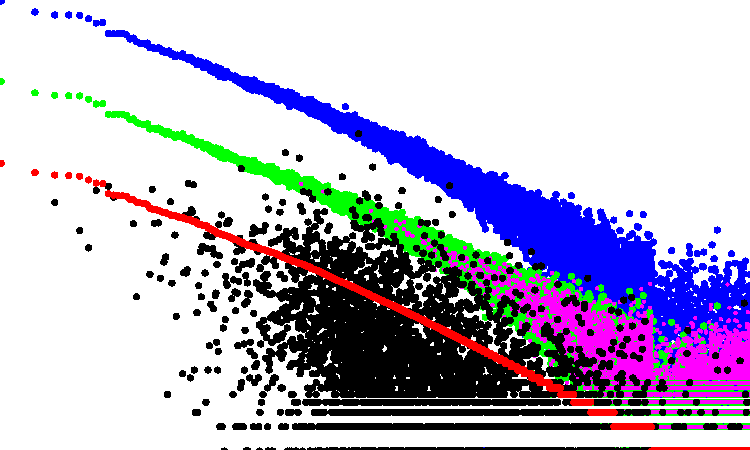
\includegraphics[width=0.95\textwidth]{ngramdata.pdf}
\end{frame}

\begin{frame}{Adding skipgram features alongside $n$-grams}

\begin{columns}[b]
            \begin{column}[b]{0.45\textwidth}
                \begin{block}{HPYLM}
                \begin{tabular}{lllllllll}
                         & jrc  & 1bw   & emea & wp   \\
                    jrc  & 3.65 & 10.22 & 9.91 & 9.98 \\
                    1bws & 9.58 & 7.31  & 9.89 & 8.94 \\
                    emea & 9.23 & 10.16 & 1.88 & 9.72 \\
                    wps  & 9.12 & 8.83  & 9.97 & 7.76 \\
                \end{tabular}
                \end{block}
                \vspace{0pt}
            \end{column}
            \quad
            \begin{column}[b]{0.45\textwidth}
                \begin{block}{Modified Kneser-Ney}
                \begin{tabular}{llll}
                    jrc  & 1bw   & emea & wp   \\
                    3.68 & 10.18 & 9.87 & 9.98 \\
                    9.55 & 7.34  & 9.85 & 8.98 \\
                    9.18 & 10.17 & 1.89 & 9.72 \\
                    9.14 & 8.88  & 9.95 & 7.82 \\
                \end{tabular}
                \end{block}
                \vspace{0pt}
            \end{column}            
        \end{columns}
 
        \begin{columns}[b]
            \begin{column}[b]{0.45\textwidth}
                \begin{block}{Relative reduction in entropy (in \%)}
                \begin{tabular}{lllll}
                    jrc  & -0.81 & 0.40  & 0.34  & 0.03  \\
                    1bws & 0.34  & -0.47 & 0.39  & -0.45 \\
                    emea & 0.51  & -0.15 & -0.41 & 0.01  \\
                    wps  & -0.31 & -0.53 & 0.21  & -0.82 \\
                \end{tabular}
                
                \end{block}
                \vspace{0pt}
            \end{column}
            \quad
            \begin{column}[b]{0.45\textwidth}
                \begin{block}{Relative reduction in perplexity (in \%)}
                \begin{tabular}{llll}
                    -2.07 & 2.80  & 2.3   & 0.23  \\
                    2.23  & -2.38 & 2.63  & -2.81 \\
                    3.20  & -1.09 & -0.54 & 0.08  \\
                    -1.98 & -3.30 & 1.43  & -4.48 \\
                \end{tabular}
                \end{block}
                \vspace{0pt}
            \end{column}            
        \end{columns}

\end{frame}

\begin{frame}{Comparing HPYLM to MKN: the Figure}
    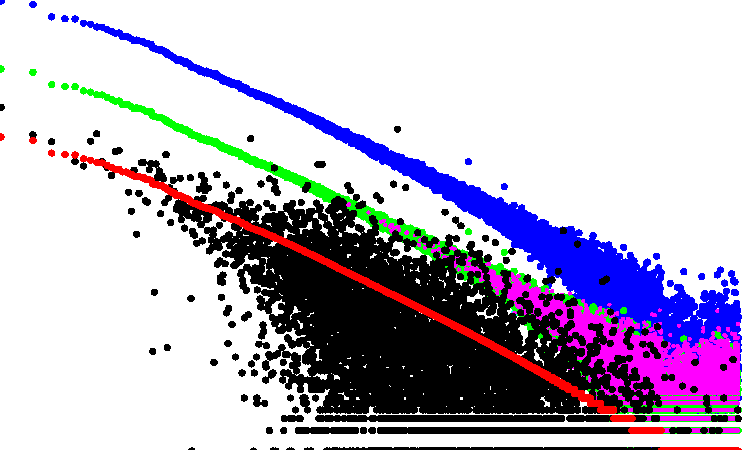
\includegraphics[width=0.95\textwidth]{sgramdata.pdf}
\end{frame}


\begin{frame}{Choosing a Language Model}
    \begin{block}{Quick turnaround}
        \begin{itemize}
        \item Modified Kneser-Ney (Kneser and Ney, 1995)
        \end{itemize}
    \end{block}
    
    \begin{block}{Best results}
        \begin{itemize}
        \item Hierarchical Pitman-Yor process language model (Teh, 2006)
        \item Recurrent neural network language model (Mikolov et al., 2010)
        \end{itemize}
\end{block}
    
    \begin{block}{Newest}
        \begin{itemize}
          \item Sparse non-negative matrix language models (Shazeer, Pelemans, and Chelba, 2014)
          \item Power low rank ensembles (Parikh et al., 2014), Gaussian embedding (Vilnis and MacCallum, under review), \ldots
       \end{itemize}
    \end{block}

\end{frame}

\end{document}

%http://stats.stackexchange.com/questions/22/bayesian-and-frequentist-reasoning-in-plain-english
